% SVN info for this file
\svnidlong
{$HeadURL$}
{$LastChangedDate$}
{$LastChangedRevision$}
{$LastChangedBy$}
% BRUTTISSIMO PUN E CHE NON È POLITICAMENTE CORRETTA; un volt m'ampere d'aver vist un'ohm che s'incoulomb un'altr'ohm. Ah Joule!
% Metalmeccanico e parrucchiere in un turbine di sesso e politica
\chapter{La circuitazione del campo magnetico, la legge di Ampère e le equazioni di Maxwell nel caso statico} 
\labelChapter{leggediampere}

\begin{introduction}
‘‘La matematica confronta i più disparati fenomeni e scopre le analogie segrete che li uniscono.''
\begin{flushright}
	\textscsl{Joseph Fourier,} cercando disperatamente di motivare ai suoi genitori la scelta di studiare matematica. %TODO: quote
\end{flushright}
\end{introduction}
\lettrine[findent=1pt, nindent=0pt]{S}{i} %TODO: intro

\section{La circuitazione del campo magnetico e legge di Ampère}
Per concludere la trattazione della magnetostatica ci rimane da descrivere la \textit{circuitazione} del campo magnetico.
\subsection{Il caso con un filo infinito}
Per capire meglio come si calcola, partiamo da un caso particolare: consideriamo un filo infinito percorso da corrente $I$ e una curva $\gamma$ che gira attorno al filo.
\begin{center}
	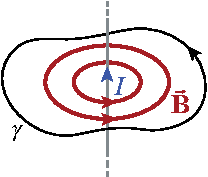
\includegraphics[width=0.45\textwidth]{images/chp9/chp9leggeampere1.pdf}
\end{center}
Tale curva è parametrizzabile in coordinate cilindriche da
\begin{equation*}
	\vba{r}'(\phi)=\left(R(\phi)\cos\phi,R(\phi)\sin\phi,z(\phi)\right)
\end{equation*}
con spostamento infinitesimo lungo la curva pari a
\begin{align*}
	d\vba{s}&=\dv{\vba{r}'(\phi)}{\phi}d\phi=\\
	&=\left[\left(R'(\phi)\cos\phi-R(\phi)\sin\phi\right)\vbh{u}_x+\left(R'(\phi)\sin\phi+R(\phi)\cos\phi\right)\vbh{u}_y+z'(\phi)\vbh{u}_z\right]d\phi=\\
	&=\left(R'(\phi)\vbh{u}_R+R(\phi)\vbh{u}_{\theta}+z'(\phi)\vbh{u}_z\right)d\phi
\end{align*}
Per la legge di Biot-Savart, in un punto a distanza $R(\phi)$ dal filo il campo magnetico è
\begin{equation*}
	\vba{B}=\frac{\mu_0 I}{2\pi R(\phi)}\vbh{u}_{\theta}
\end{equation*}
Osserviamo che nel prodotto scalare $\vba{B}\vdot d\vba{s}$ si ha
\begin{equation*}
	\begin{cases}
		\vbh{u}_\theta\vdot\vbh{u}_R=0\\
		\vbh{u}_\theta\vdot\vbh{u}_z=0
	\end{cases}
\end{equation*}
La circuitazione del campo magnetico, in questo caso, è
\begin{equation*}
	\Gamma_{\gamma}(\vba{B})=\int_{\gamma}\vba{B}\vdot d\vba{s}=\int_{\gamma}\frac{\mu_0 I}{2\pi}d\phi=\mu I
\end{equation*}
\begin{equation}
	\Gamma_{\gamma}(\vba{B})=\oint \vba{B}\vdot d\vba{s}=\mu_0 I
\end{equation}
\subsection{Il caso con due fili infiniti}
Supponiamo ora di avere, all'interno della stessa curva di prima, due fili rettilinei infiniti invece che uno. Per descrivere la circuitazione in questo caso introduciamo un segmento immaginario orientato $\eta$ tra i due fili che colleghi due punti del circuito, in modo da dividere la curva $\gamma$ in due sotto-curve $\xi_1$ e $\xi_2$.
\begin{center}
	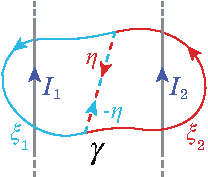
\includegraphics[width=0.45\textwidth]{images/chp9/chp9leggeampere2.pdf}
\end{center}
Allora, possiamo definire due curve chiuse
\begin{align*}
	\gamma_1=\xi_1 \cup \left(-\eta\right)&&\gamma_2=\xi_2\cup \eta 
\end{align*} 
dove $-\eta$ è il segmento $\eta$ percorso nel verso opposto. Si osservi che
\begin{equation*}
	\gamma_1\cup\gamma_2=\xi_1\cup \left(-\eta\right)\cup \xi_2\cup \eta=\xi_1\cup \xi_2=\gamma
\end{equation*}
dato che i segmenti orientati si elidono a vicenda. Allora, dato nell'interno dell'area delimitata dalle curve $\gamma_i$ passa un solo filo, vale il caso precedente e quindi 
\begin{equation}
	\Gamma_{\gamma}(\vba{B})=\Gamma_{\gamma_1}(\vba{B})+\Gamma_{\gamma_2}(\vba{B})=\mu_0 I_1+\mu_0I_2
\end{equation}
dove $I_j$ sono presi con segno: se si fissa un segno di percorrenza, il verso di percorrenza ha segno opposto - ad esempio, se la corrente è antioraria il segno è positivo, negativo se oraria.
\subsection{Il caso generale: legge (della circuitazione) di Ampère}
\begin{theorema}[Legge {(della circuitazione)} di Ampère]\index{legge!(della circuitazione) di Ampère}
	Dato un campo magnetico $\vba{B}$ generato da della corrente $I$, la circuitazione do $\vba{B}$ lungo una curva chiusa $\gamma$ è proporzionale alla porzione di corrente $I_{int}$ che attraversa una qualunque superficie $\Sigma$ con bordo la curva (cioè tale per cui $\gamma=\partial\Sigma$).
	\begin{itemize}
		\item \textbf{Forma integrale:}
		\begin{equation}
			\Gamma_{\gamma}(\vba{B})=\oint_{\partial \Sigma} \vba{B}\vdot d\vba{s}=\mu_0\int_{\Sigma}\vba{j}\vdot\vbh{u}_nd\Sigma=\mu_0 I_{int}\label{LeggeAmpereMagnetostaticaIntegrale}
		\end{equation}
		\item \textbf{Forma differenziale:}
		\begin{equation}
			\curl{\vba{B}}=\mu_0\vba{j}\label{LeggeAmpereMagnetostaticaDifferenziale}\qedhere
		\end{equation}
	\end{itemize}
\end{theorema}
\begin{demonstration}
	Deriviamo la forma differenziale. Per il teorema del rotore vale
	\begin{equation*}
		\Gamma_{\gamma}(\vba{B})=\oint_{\partial \Sigma} \vba{B}\vdot d\vba{s}=\int_{\Sigma}\curl{\vba{B}}\vdot\vbh{u}_nd\Sigma=\Phi_{\Sigma}\left(\curl{\vba{B}}\right)
	\end{equation*}
	Ma allora, valendo l'uguaglianza
	\begin{equation*}
		\int_{\Sigma}\curl{\vba{B}}\vdot\vbh{u}_nd\Sigma=\mu_0\int_{\Sigma}\vba{j}\vdot\vbh{u}_n
	\end{equation*}
	per una qualunque superficie $\Sigma$ arbitraria, si ha l'identità delle integrande:
	\begin{equation*}
		\curl{\vba{B}}=\mu_0\vba{j}\qedhere
	\end{equation*}
\end{demonstration}
Questa non è altro che l'ultima \textit{equazione di Maxwell} (su quattro) che ci mancava per i fenomeni elettromagnetici non dipendenti dal tempo, sebbene nella meno elegante forma integrale.
\subparagraph{Un cavillo della legge di Ampère}
%Un primo cavillo di questo teorema sta nell'ambiguità di segno. Ci sono tre termini che dipendono dal segno: l'integrale lungo $\gamma$, dato che è una curva orientata, il versore $\vba{u}_n$ normale alla superficie e la corrente $I_{int}$ che attraversa $\Sigma$. In tal caso, ci affida ad un'altra versione della mano destra: posto il palmo della mano destra rispetto all'area di integrazione e puntato l'indice nel verso dello spostamento infinitesimo, il pollice
% https://en.wikipedia.org/wiki/Amp%C3%A8re%27s_circuital_law, ma che cazzo di verso viene il versore normale?
Si osservi che la legge appena trovata è valida soltanto se la corrente è \textit{stazionaria}, ossia se è \textit{costante} nel tempo. Per capire perché, ricordiamo che la \textit{divergenza di un rotore} è sempre nulla:\label{laleggediAmpereèfalsaepretenziosa}
\begin{equation*}
	\div{\left(\curl{\vba{B}}\right)}=0
\end{equation*}
Se la nostra legge fosse corretta, si avrebbe
\begin{equation*}
	0=\div{\left(\curl{\vba{B}}\right)}=\mu_0\div{\vba{j}}=-\pdv{\rho}{t}
\end{equation*}
dove nell'ultimo passaggio abbiamo fatto uso dell'\textit{equazione di continuità}:
\begin{equation*}
	\div{\vba{j}}+\pdv{\rho}{t}=0
\end{equation*}
Di conseguenza, si avrebbe
\begin{equation*}
	\pdv{\rho}{t}=0
\end{equation*}
ma ciò è vero soltanto per una corrente stazionaria!\\
Da ciò capiamo la legge di Ampère per la circuitazione \textit{non} è sempre corretta nella forma di cui sopra; sarà necessario integrarla con un altro termine che tiene conto della \textit{variazione temporale} della corrente - ma questa è una storia per un altro capitolo.
\paragraph{⋆ Tra astratto e concreto: teoria dei nodi nella legge di Ampère}
Ci sono aspetti della Matematica che per un fisico risultano spesso astrusi, \textit{astratti} e lontani dalla realtà; eppure, in alcuni casi il passo tra il mondo concreto e la Matematica teorica è più \textit{breve} di quel che sembra. Possiamo vedere un esempio di ciò nella \textit{dimostrazione della legge di Ampère} nella sua forma generale.
\begin{demonstrationwtnoqed}[Parte prima]
Vogliamo calcolare la circuitazione del campo magnetico $\vba{B}$ generato da un circuito chiuso qualunque $\gamma_2$ 
\begin{equation*}
	\Gamma_{\gamma_1}(\vba{B})=\oint_{\gamma_1}\vba{B}\vdot d\vba{s}
\end{equation*}
Parametrizziamo le due curve $\gamma_i$ con angoli $\phi_i$:
\begin{align*}
	\gamma_1\colon \vba{r}_1=\vba{r}_1(\phi_1) && 
	\gamma_2\colon \vba{r}_2=\vba{r}_2(\phi_2)
\end{align*}
Lo spostamento infinitesimo lungo la curva $\gamma_i$ è
\begin{equation*}
	d\vba{s}_i=\dv{\vba{r}_i(\phi_i)}{\phi_i}d\phi_i
\end{equation*}
Per la prima legge di Laplace il campo generato dal circuito $\gamma_2$ è
\begin{equation*}
	\vba{B}=\frac{\mu_0 I}{4\pi}\oint_{\gamma_2}d\vba{s}_2\cross\frac{\vba{r}-\vba{r}_2(\phi_2)}{\abs{\vba{r}-\vba{r}_2(\phi_2)}^3}
\end{equation*}
La circuitazione $\vba{B}$ lungo la curva $\gamma_2$ si calcola tenendo conto che $\vba{B}$ deve essere valutato sull'altra curva, ossia prendendo $B(r(\phi_1))$: 
\begin{align*}
	\Gamma_{\gamma_1}(\vba{B})&=\frac{\mu_0 I}{4\pi}\oint_{\gamma_1} \oint_{\gamma_2} \left(d\vba{s}_2 \cross \frac{\vba{r}_1(\phi_1) - \vba{r}_2(\phi_2)}{\abs{\vba{r}1(\phi_1) - \vba{r}_2(\phi_2)}^3}\right) \vdot d\vba{s}_1=\\
	&=\frac{\mu_0 I}{4\pi}\oint_{\gamma_1} \oint_{\gamma_2} \frac{\vba{r}_1(\phi_1) - \vba{r}_2 (\phi_2)}{\abs{\vba{r}_1(\phi_1) - \vba{r}_2(\phi_2)}^3} \vdot \left(d\vba{s}_1\cross d\vba{s}_2\right)
\end{align*}
dove abbiamo applicato la proprietà del prodotto misto
\begin{equation*}
	\vba{a}\vdot\left(\vba{b}\cross\vba{c}\right)=
	\vba{b}\vdot\left(\vba{c}\cross\vba{a}\right)=
	\vba{c}\vdot\left(\vba{a}\cross\vba{b}\right)
\end{equation*}
La cosa peculiare è il doppio integrale curvilineo che abbiamo trovato, diviso per $4\pi$, è pari al \textbf{linking number di Gauss} (in italiano \textit{numero di concatenamento}), un \textit{invariante numerico} rilevante con teoria dei nodi.
\end{demonstrationwtnoqed}
Matematicamente parlando, una curva chiusa nello spazio tridimensionale è quello che definiamo come \textbf{nodo}.
\begin{define}[Nodo]
	Un \textbf{nodo}\index{nodo} è un'inclusione topologica $\funz[f]{S^1}{\realset^3}$ della circonferenza $S^1$ in $\realset^3$, cioè se $\funz[f]{S^1}{f(S^1)}$ è un omeomorfismo.
\end{define}
I nodi possono essere proiettati su un piano $\realset^2$; tale proiezione è quasi sempre \textbf{regolare}, ossia che è iniettiva sempre tolto al più un numero finito di incroci, proiezione di soli due punti del nodo.
\begin{define}[Mappa di Gauss]
	Dati due nodi differenziabili $\funz[f]{S^1}{\realset^3}$, la \textbf{mappa di Gauss}\index{mappa!di Gauss} è la funzione
	\begin{equation}
		\funztot[G(\phi_1,\phi_2)]{S^1\times S^1}{S^2}{\left(\phi_1,\phi_2\right)}{\frac{\vba{r}_1(\phi_1) - \vba{r}_2 (\phi_2)}{\abs{\vba{r}_1(\phi_1) - \vba{r}_2(\phi_2)}}}
	\end{equation}
	Dato che la mappa non è biunivoca, la mappa può ricoprire la sfera più volte.
\end{define}
\begin{define}[Linking number di Gauss]
	Il \textbf{linking number di Gauss} è un numero intero che conta quante volte due nodi si avvolgono tra di loro - senza intersecarsi direttamente. Il segno di tale numero dipende dall'orientazione scelta delle due curve.\\
	Formalmente, esso corrisponde a quante volte con segno l'immagine di $G$ ricopre la sfera $S^2$:
	\begin{align}
		\textrm{lk}(\gamma_1,\gamma_2)=&\frac{1}{4\pi}\frac{1}{4\pi}\oint_{\gamma_1} \oint_{\gamma_2} \frac{\vba{r}_1(\phi_1) - \vba{r}_2 (\phi_2)}{\abs{\vba{r}_1(\phi_1) - \vba{r}_2(\phi_2)}^3} \vdot \left(d\vba{s}_1\cross d\vba{s}_2\right)\\
		=&\frac{1}{4\pi}\int_{S^1\times S^1}\frac{\det\left(\vbd{r}_1(\phi_1),\vbd{r}_2(\phi_2),\vba{r}_1(\phi_1)-\vba{r}_2(\phi_2)\right)}{\abs{\vba{r}_1(\phi_1) - \vba{r}_2(\phi_2)}}d\phi_1d\phi_2
	\end{align}
	Il doppio integrale curvilineo qui scritto è l'area totale con segno dell'immagine di $G$, che va diviso per l'area della sfera unitaria.
\end{define}
\begin{example}~
	\begin{itemize}
		\item $\textrm{lk}(\gamma_1,\gamma_2)=\pm 1$
		\begin{center}
			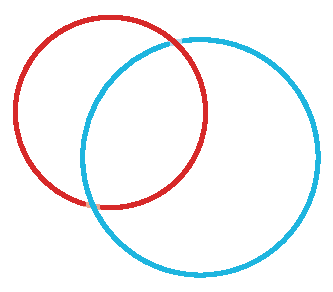
\includegraphics[width=0.25\textwidth]{images/chp9/chp9linknumb1.pdf}
		\end{center}
		\item $\textrm{lk}(\gamma_1,\gamma_2)=\pm 2$
		\begin{center}
			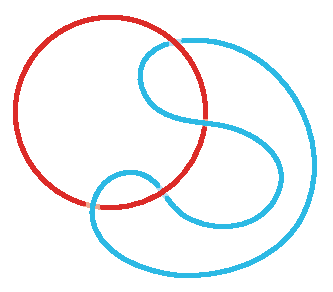
\includegraphics[width=0.25\textwidth]{images/chp9/chp9linknumb2.pdf}
		\end{center}
	\end{itemize}
\end{example}
Possiamo adesso concludere la dimostrazione iniziata precedentemente.
\begin{demonstrationwt}[Parte seconda]
La circuitazione del campo magnetico lungo una curva si può quindi scrivere in funzione del linking number della curva lungo cui si calcola e del circuito che genera il campo:
\begin{equation*}
	\Gamma_{\gamma_1}(\vba{B})=\mu_0 I\ \textrm{lk}(\gamma_1,\gamma_2)
\end{equation*}
A seconda di quante volte il circuito e la curva si avvolgono, la corrente interna alla curva $I_{int}$ non è necessariamente $I$: essa può essere pari a multipli interi (con segno) della corrente $I$. Tale valore, per l'appunto, lo otteniamo con il linking number, ottenendo così la legge di Ampère nel caso generale.
\end{demonstrationwt}
\paragraph{Applicazioni della legge di Ampère}
Adesso useremo la legge di Ampère per ricavare il \textit{campo magnetico}, in modo analogo a come si può ricavare in casi di particolari simmetrie il \textit{campo elettrico} con la \textit{legge di Gauss}.
\begin{examplewt}[Legge di Biot-Savart per un filo rettilineo infinito]
	Consideriamo un filo rettilineo infinito. Per simmetria il campo magnetico è dipendente solo dalla distanza assiale dal filo d è diretto lungo $\vbh{u}_\theta$, tangenziale a delle circonferenze centrate lungo il filo. Poste le coordinate cilindriche
	\begin{equation*}
		\begin{cases}
			x=R\cos\theta\\
			y=R\sin\theta
		\end{cases}
	\end{equation*}
	si ha
	\begin{equation*}
		\vba{B}=B(R)\vbh{u}_\theta
	\end{equation*}
	Poniamoci lungo una curva immaginaria su cui $\vba{B}$ è costante, ad esempio una circonferenza $\gamma$ di raggio $R$ centrata nel filo. In questo caso lo spostamento infinitesimo lungo tale curva è
	\begin{equation*}
		d\vba{s}=R\vbh{u}_\theta d\theta
	\end{equation*}
	Allora, usando la legge di Ampère, si ha
	\begin{equation*}
		\mu_0I=\Gamma_{\gamma}(\vba{B})=\oint\vba{B}\vdot d\vba{s}=\oint B(R)R\vbh{u}_\theta\vdot\vbh{u}_{\theta}d\theta=B(R)R\int_{0}^{2\pi}d\theta=2\pi R B(R)
	\end{equation*}
	da cui
	\begin{equation}
		B(R)=\frac{\mu_0 I}{2\pi R}
	\end{equation}
\end{examplewt}

\begin{examplewt}[Solenoide infinito]
	%Per simmetria, il solenoide infinito produce un campo magnetico all'interno del solenoide e nessun campo magnetico all'esterno del solenoide stesso. Proviamo a ricavarlo di nuovo usando una particolare curva.\\
	Consideriamo un solenoide di lunghezza infinita, posto lungo l'asse verticale $z$. Per calcolare il campo magnetico all'interno (all'esterno è nullo), prendiamo una curva $\gamma=\overrightarrow{ABCD}$ rettangolare e calcolo la circuitazione lungo essa. Tale curva è costituita da quattro tratti:
	\begin{itemize}
		\item $\overrightarrow{AB}$ è un segmento verticale \textit{interno} al solenoide, diretto verso l'alto.
		\item $\overrightarrow{BC}$ è un segmento orizzontale, intersecante il solenoide e diretto verso l'esterno.
		\item $\overrightarrow{CD}$ è un segmento verticale \textit{esterno} al solenoide, diretto verso il basso.
		\item $\overrightarrow{DA}$ è un segmento orizzontale, intersecante il solenoide e diretto verso l'interno.
	\end{itemize}
	\begin{center}
		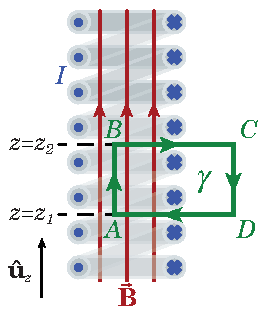
\includegraphics[width=0.45\textwidth]{images/chp9/chp9solenoidecircuitazione.pdf}
	\end{center}
	La circuitazione lungo la curva $\gamma$ sarà
	\begin{align*}
		\Gamma_{\gamma}(\vba{B})=&=\oint\vba{B}\vdot d\vba{s}=\left( \int_A^B + \int_B^C + \int_C^D + \int_D^A  \right) \vba{B}\vdot d\vba s= \int^B_A \vba{B}\vdot s=\\
		&=\int_{A}^{B}\vba{B}\vdot d\vba{s}=\int^{z_2}_{z_1} B(R)dz=B(R)(z_2-z_1)
	\end{align*}
	dove $z_1$ è la quota di $A$ e $z_2$ quella di $B$. Infatti, tutti gli altri contributi sono nulli:
	\begin{itemize}
		\item I contributi della circuitazione lungo  $\overrightarrow{BC}$ e $\overrightarrow{DA}$ sono nulli perché perpendicolari al campo.
		\item Il contributo della circuitazione lungo $\overrightarrow{CD}$ è nullo perché all'esterno del solenoide non c'è campo.
	\end{itemize}
	Per la legge di Ampère
	\begin{equation*}
		\Gamma_{\gamma}(\vba{B})=\mu_0I_\gamma
	\end{equation*}
	dove $I_\gamma$ è corrente che attraversa la curva $\gamma$, che dipende dal numero di spire $N$ contenute all'interno di $\gamma$:
	\begin{equation*}
		N=\int_{z_1}^{z_2}ndz=n\left(z_2-z_1\right)
	\end{equation*}
	dove $n$ è la densità lineare di spire, che supponiamo costante. Allora
	\begin{equation*}
		I_{\gamma}=N I = n\left(z_2-z_1\right) I
	\end{equation*}
	dove $I$ è la corrente in una singola spira. Concludiamo che
	\begin{equation*}
		B(R)\Ccancel[red]{(z_2-z_1)}=\Gamma_{\gamma}(\vba{B})=\mu_0I_\gamma=n\Ccancel[red]{(z_2-z_1)} I
	\end{equation*}
	\begin{equation}
		B(R)=\mu_0 n I
	\end{equation}
	Come già osservato il campo del solenoide non dipende dalla distanza assiale, ma è uniforme in \textit{tutto} il solenoide. 
\end{examplewt}
\section{Equazioni di Maxwell per l'elettrostatica e la magnetostatica}
%TODO: FORSE SPOSTARE CAPITOLO NUOVO
\begin{center}
	\begin{tabular}{p{0.2\textwidth}|c|c}
		%\multicolumn{2}{c}{\textbf{---}} \\\hline  >{\centering}
		\centering{\textbf{Nome}} &
		\textbf{Forma integrale} &
		\begin{tabular}{@{}c@{}} \textbf{Forma} \\ \textbf{differenziale}\end{tabular} \\ \hline
		
		\begin{tabular}[c]{@{}p{0.2\textwidth}@{}}	
			\\[-3mm] \textbf{Legge di Gauss per l'elettricità}
		\end{tabular}
		&
		\begin{tabular}[c]{@{}c@{}}
			\\[-3mm]
			$\displaystyle\Phi_{\partial V}(\vba{E})=\int_{\partial V}\vba{E}\vdot\vbh{u}_nd\Sigma=\frac{q_{int}}{\epsilon_0}=\frac{1}{\epsilon_0}\int_{V}\rho dV$
		\end{tabular} &
		\begin{tabular}[c]{@{}c@{}}
			\\[-3mm]
			$\displaystyle\div{\vba{E}}=\frac{\rho}{\epsilon_0}$
		\end{tabular} \\ \hline
		\begin{tabular}[c]{@{}p{0.2\textwidth}@{}}	
			\\[-3mm] \textbf{Legge di Gauss per il magnetismo}
		\end{tabular} &
		\begin{tabular}[c]{@{}c@{}}
			\\[-3mm]
			$\displaystyle\Phi_{\partial V}(\vba{B})=\int_{\partial V}\vba{B}\vdot\vbh{u}_nd\Sigma=0$
		\end{tabular} &
		\begin{tabular}[c]{@{}c@{}}
			\\[-3mm]
			$\displaystyle\div{\vba{B}}=0$
		\end{tabular} \\ \hline
		\begin{tabular}[c]{@{}p{0.2\textwidth}@{}}	
			\\[-3mm] \textbf{Legge dell'induzione di Faraday}
		\end{tabular} &
		\begin{tabular}[c]{@{}c@{}}
			\\[-3mm]
			$\displaystyle\Gamma_{\partial \Sigma}(\vba{E})=\oint_{\partial \Sigma}\vba{E}\vdot d\vba{s}=0$
		\end{tabular}	
		&
		\begin{tabular}[c]{@{}c@{}}
			\\[-3mm]
			$\displaystyle\curl{\vba{E}}=0$
		\end{tabular} \\ \hline
		\begin{tabular}[c]{@{}p{0.18\textwidth}@{}}	
			\\[-3mm] \textbf{Legge della circuitazione di Ampère}
		\end{tabular} &
		\begin{tabular}[c]{@{}c@{}}
			\\[-3mm]
			$\displaystyle\Gamma_{\partial \Sigma}(\vba{B})=\oint_{\partial \Sigma}\vba{B}\vdot d\vba{s}=\mu_0\int_{\Sigma}\vba{j}\vdot\vbh{u}_n=\mu_0 I_{int}$
		\end{tabular} &
		\begin{tabular}[c]{@{}c@{}}
			\\[-3mm]
			$\displaystyle\curl{\vba{B}}=\mu_0\vba{j}$
		\end{tabular}
	\end{tabular}
\end{center}
\begin{observe}
	Sebbene le \textit{leggi di Gauss} per l'\textit{elettricità} e per il \textit{magnetismo} siano valide anche se i campi elettrici e magnetici sono variabili nel tempo, lo stesso non si può dire per le \textit{leggi di Faraday} e di \textit{Ampère}: dovremo aggiungere a ciascuna un opportuno termine \textit{dipendente dal tempo}.\\
	Una conseguenza di ciò che esploreremo meglio successivamente è che il campo elettrico dipendente dal tempo \textit{non} è più conservativo; il campo magnetico, invece, resta sempre solenoidale.
\end{observe}
\subsection{Invarianza di gauge nell'elettromagnetostatica}\label{invarianzagauge}
Nel \autoref{chap:PotenzialeElettrico}, sezione \ref{EqPoissonSezione}, abbiamo parlato delle equazioni di Poisson e di Laplace:
\begin{itemize}
	\item \textbf{Equazione di Poisson} (caso non omogeneo, $\rho\neq 0$):
	\begin{equation}
		\laplacian{V}=-\frac{\rho}{\epsilon_0}
	\end{equation}
	\item \textbf{Equazione di Laplace} (caso omogeneo, $\rho=0$):
	\begin{equation}
		\laplacian{V}=0
	\end{equation}
\end{itemize}
Qui $V$ è il \textit{potenziale scalare} del campo elettrostatico $\vba{E}$ tale per cui $\vba{E}=-\grad{V}$, mentre $\rho$ è la densità di carica.

Un'equazione differenziale simile si può scrivere per il campo magnetico.		Siccome la divergenza del campo magnetico è nulla per la legge di Gauss, allora esiste un potenziale vettore $\vba{A}$ tale che $\vba{B}=\curl{\vba{A}}$. Sostituendo questa equazione nella \textit{legge di Ampère} otteniamo
\begin{equation*}
	\curl\left(\curl\vba{A}\right)=\mu_0\vba j
\end{equation*}
che, sviluppando, risulta
\begin{equation*}
	\grad \left( \div{\vba{A}}\right) - \laplacian{\vba{A}}=\mu_0 \vba j
\end{equation*}
Ci è oramai ben noto che il potenziale scalare $V$ è sempre definito a \textit{meno di costante}. Infatti, quello che conta - anche dal punto di vista fisico - è la \textit{differenza di potenziale}. In termini più rigorosi, quando parliamo del potenziale quello che stiamo facendo è prendere un opportuno \textit{rappresentante} dalla classe di equivalenza $\left[V\right]$, ottenuta dalla relazione
\begin{align*}
	V\sim V+a \qquad \text{dove}\ a\in\realset
\end{align*}
Nel caso del vettore potenziale si verifica una situazione analoga. Data una \textit{funzione scalare} $\oldphi$, $\vba{A}$ è definito \textit{a meno di gradiente}. In termini di classi di equivalenza, $\vba{A}$ è il rappresentante della classe $[\vba{A}]$ data dalla relazione
\begin{align*}
	\vba{A}\sim \vba{A}+\grad{\phi} \qquad \text{dove}\ \funz[\phi]{\realset^3}{\realset}
\end{align*}
Infatti, si vede che il campo magnetico resta invariato:
\begin{equation*}
	\vba{B}=\curl\vba{A}=\curl \left( \vba{A}+\grad\oldphi\right)= \curl \vba{A} + \Ccancel[red]{\curl\grad\oldphi}=\curl\vba{A}		
\end{equation*}
In particolare ciò succede perché il rotore del gradiente è nullo.\\
In sostanza, abbiamo descritto un caso di \textbf{invarianza di gauge}\index{gauge!invarianza di}.
\begin{define}[Invarianza di gauge]
	Consideriamo una configurazione elettromagnetica $\left(\vba{E},\vba{B}\right)$ e supponiamo che essa sia descritta dai campi potenziali $\left(V,\vba {A}\right)$. Allora esiste una trasformazione arbitraria $\Lambda=$, detta \textbf{trasformazione (locale) di gauge}\index{gauge! trasformazione di}, tale da ottenere una \textit{nuova} coppia di campi potenziali $\left(V',\vba {A}'\right)$...
	\begin{align*}
		V\overset{\Lambda}{\longleftrightarrow} V'=V+c\\
		\vba{A}\overset{\Lambda}{\longleftrightarrow} \vba{A}'=\vba{A}+\grad{\phi}
	\end{align*}
	... che descrive la \textit{stessa} configurazione $\left(\vba{E}',\vba{B}'\right)=\left(\vba{E},\vba{B}\right)$. i campi elettrici e magnetici sono \textit{invarianti di Gauge}\index{gauge!invarianti di}.
\end{define}
Questo distingue profondamente ciò che è effettivamente osservabile da ciò che non lo è, almeno direttamente. I campi elettrici e magnetici sono \textit{osservabili} direttamente e hanno un particolare valore. I campi \textit{potenziali} elettrici e magnetici sono meglio descrivibili come \textit{classi di equivalenza}; dato che non possiamo parlare di un rappresentante preferito, a priori \textit{non} è possibile osservarli direttamente senza fare una scelta particolare del rappresentante. Tale scelta è detta \textbf{scelta di gauge}\index{gauge!scelta di}
\begin{intuit}
	Guardando un asta perfettamente cilindrica è possibile dire se è attorcigliata o no? A priori no: ciascuna sezione ortogonale del cilindro è uguale - o per meglio dire \textit{invariante} - rispetto ad ogni potenziale simmetria circolare del cilindro. Tuttavia, se lungo l'asta disegnassimo una linea dritta, allora potremmo determinare se il cilindro è contorto o no, dato che basta guardare com'è la linea.\\
	In modo analogo, l'asta corrisponde al campo elettromagnetico e lo status di ‘‘essere attorcigliata'' ai campo potenziali: la linea dritta corrisponde ad una scelta di gauge, dato che le sezioni ortogonali non sono invarianti per le simmetrie circolari.
\end{intuit}
\noindent Fare una scelta certamente rovina l'invarianza di gauge, ma ci permette spesso di ricondurci ad una situazione molto più facile da studiare.\\
Ad esempio, supponiamo di avere un campo potenziale magnetico $\vba{A}$ tale per cui $\div{\vba{A}}\neq 0$. Possiamo effettuare una \textit{scelta di gauge} imponendo che la trasformazione descritta dal campo scalare $\oldphi$, ossia
\begin{equation*}
	\vba{A}\mapsto\vba{A}'=\vba{A}+\grad{\oldphi},
\end{equation*}
sia tale per cui $\div{\vba{A}'}=0$. Questa condizione si scrive come
\begin{gather*}
	\div\vba{A}+\div\grad\oldphi=0 \implies \laplacian\oldphi= -\div\vba{A}
\end{gather*}
In questo modo $\oldphi$ sarà determinato da un'equazione differenziale del secondo ordine.

Preso allora $\vba{A}$ con la scelta di gauge qui sopra, dato che $\div{A}=0$ si ha $\grad{\left(\div{A}\right)}=0$, da cui segue
\begin{equation*}
	\grad \left( \div{\vba{A}}\right) - \laplacian{\vba{A}}=\mu_0 \vba j\implies \laplacian{\vba{A}}=-\mu_0 \vba j
\end{equation*}
Previa una scelta di gauge opportuna, l'intera elettromagnetostatica può essere descritta da quattro equazioni di Laplace - una con il potenziale scalare per l'elettrostatica, e tre con il potenziale vettoriale per la magnetostatica.
\begin{align}
	\laplacian A_x&=\mu_0 j_x\\
	\laplacian A_y&=\mu_0 j_y\\
	\laplacian A_z&=\mu_0 j_z\\
	\laplacian V&=-\frac{\rho}{\epsilon_0}
\end{align}
La soluzione più generale di queste equazioni differenziali, date le \textit{condizioni al contorno} di natura fisica
\begin{equation*}
	V,\ \vba{A}\underset{\vba{r}\to\infty}{\to}0
\end{equation*}
è data da
\begin{align}
	\vba{A}(\vba r)&=\frac{\mu_0}{4\pi}\int\frac{\vba j(\vba r')}{\abs{\vba r-\vba r'}} dV'\\
	V(\vba r)&=\frac{1}{4\pi\epsilon_0}\int \frac{\rho(\vba r')}{\abs{\vba r-\vba r'}}dV'
\end{align}
dove $dV'=dx'dy'dz'$.
Noti dunque $\rho$ e $\vba{j}$ siamo in grado descrivere completamente una configurazione (statica) di natura elettromagnetica - modulo saper calcolare l'integrale, che non è per nulla scontato.
\begin{examplewt}[Sfera carica uniformemente]
	Ricalcoliamo\footnote{Avevamo calcolato il potenziale elettrostatico in presenza di simmetria radiale direttamente a partire dalle equazioni di Poisson e Laplace nel \autoref{chap:PotenzialeElettrico}, sezione \ref{EquazioniPoissonSimmetriaSferica}, pag. \pageref{EquazioniPoissonSimmetriaSferica}; per ottenere nello specifico il caso della \textit{sfera carica}  avevamo imposto le condizioni al contorno solo successivamente. Il procedimento qui scelto risulta utilizza invece la soluzione scritta poc'anzi - ma di fatto l'origine è anch'essa dalle equazioni di Laplace e Poisson} il campo elettrico interno ed esterno ad una sfera di raggio $r_0$ carica uniformemente con densità di carica
	\begin{equation*}
		\rho(\vba r)=
		\begin{cases}
			\rho & r<r_0\\
			0 & r>r_0
			\end{cases}=\rho\xi_{[0,r_0]}
	\end{equation*}
	Prese le coordinate sferiche
	\begin{equation*}
		\begin{cases}
			x=r\cos\phi\sin\theta\\
			y=r\sin\phi\sin\theta\\
			z=r\cos\theta
		\end{cases}
	\end{equation*}
	l'elemento di volume risulta
	\begin{equation*}
		dV=r^2\sin\theta drd\theta d\phi
	\end{equation*}
	mentre la differenza di coordinate tra un punto generico $\vba{r}$ e il vettore posizione d'integrazione  $\vba{r}'$ è
	\begin{equation*}
		\abs{\vba r-\vba r'}=\sqrt{r^2+(r')^2-2rr'\cos\theta '}
	\end{equation*}
	Il dominio di integrazione della variabile $r$ sarebbe definito fra $0$ e $+\infty$, ma siccome $\rho$ è \textit{non} nullo solo all'interno della sfera ci limitiamo , come indicato dalla funzione indicatrice $\xi_{[0,r_0]}$, tra $0$ e $r_0$. Inoltre, supponendo $\rho$ si può portar fuori dall'integrale ottenendo
	\begin{equation*}
		V(r)=\frac{\rho}{4\pi\epsilon_0}\int^{r_0}_0dr' \int^\pi_0 d\theta' \int^{2\pi}_0 d\phi' \frac{(r')^2 \sin\theta '}{\sqrt{r^2+(r')^2 -2rr'\cos\theta '}}\squarequal	
	\end{equation*}
	%NOTA: l'itemize è una mia idea per riassumere tutte le varie considerazioni, in un testo unico sarebbe stato un po' dispersivo e sembrava un essay in cui si cercano 100 sinonimi di since
	% nice idea, per la prima parte
	Operiamo il cambio di variabile $u=\cos\theta'$: il differenziale diventa $du=-\sin\theta'd\theta'$ e gli estremi di integrazione rispetto a $u$ sono $\pm 1$.
	\begin{align*}
		\squarequal&\frac{\rho}{2\epsilon_0}\int^{r_0}_0 \negthickspace dr'\int^1_{-1}\negthickspace du \frac{-(r')^2}{\sqrt{r^2+(r')^2-2rr'u}}=\\
		=&\frac{\rho}{2\epsilon_0}\int^{r_0}_0 \negthickspace dr' \eval{\frac{-(r')^{\Ccancel[red]{2}}}{r\Ccancel[red]{r'}} \sqrt{r^2+(r')^2-2rr'u}}^1_{-1}=\\
		=&\frac{\rho}{2\epsilon_0r}\int^{r_0}_0 dr'\ -r'\left(\sqrt{r^2+(r')^2-2rr'}-\sqrt{r^2+(r')^2+2rr'}\right)=\\
		=&\frac{\rho}{2\epsilon_0r}\int^{r_0}_0 dr'\ r'\left(\sqrt{\left(r+r'\right)^2}-\sqrt{\left(r-r'\right)^2}-\right)=\\
		=&\frac{\rho}{2\epsilon_0r}\int^{r_0}_0 dr'\ r'\left(\abs{r+r'}-\abs{r-r'}\right)=\\
		=&=\frac{\rho}{2\epsilon_0r}\int^{r_0}_0 dr'\ r'\left( r+r' + \abs{r-r'} \right)
	\end{align*}
	Adesso distinguiamo il caso \textit{esterno} ed \textit{interno} alla sfera.
	\begin{itemize}
		\item \textbf{Fuori dalla sfera} ($r>r_0$). Dato che $0<r'<r_0$ per gli estremi di integrazione, consideriamo $r>r'$; segue che $\abs{r-r'}=r-r'$ e dunque
		\begin{equation*}
			V(r)=\frac{\rho}{\Ccancel[red]{2}\epsilon_0 r}\int^{r_0}_0 \Ccancel[red]{2} (r')^2 dr'= \frac{\rho r_0^3}{3\epsilon_0 r}\squarequal
		\end{equation*}
		Siccome $\rho$ è la densità di carica della sfera, cioè
		\begin{equation*}
			\rho=\frac{q}{V_S}=\frac{q}{\frac{4}{3} \pi r_0^2}
		\end{equation*}
		dove $q$ è la carica distribuita sul volume della sfera $V_S$, sostituendo troviamo il solito potenziale di Coulomb:
		\begin{equation*}
			\squarequal\frac{q\Ccancel[red]{r_0^3}}{\frac{4}{\Ccancel[red]{3}}\Ccancel[red]{3}\pi \Ccancel[red]{r_0^3} r}=\frac{q}{4\pi \epsilon_0 r}
		\end{equation*}
		\begin{equation}
			V(r)=\frac{\rho r_0^3}{3\epsilon_0 r}=\frac{q}{4\pi \epsilon_0 r}
		\end{equation}
		Il campo elettrico associato è
		\begin{equation}
			\vba{E}(\vba{r})=-\grad V=\pdv{V}{r}\vbh{u}_r =\frac{q}{4\pi\epsilon_0 r^2}\vbh{u}_r
		\end{equation}
		\item \textbf{Dentro la sfera} ($r<r_0$). Dobbiamo spezzare l'integrale in due a seconda del segno del modulo: in $\left[0,r\right]$ e in $\left[r, r_0\right]$.
		\begin{align*}
			V(r)&=\frac{\rho}{2\epsilon_0}\left( \int^r_0 dr'(2r')^2 + \int^{r_0}_r dr' 2rr' \right)= \frac{\rho}{2\epsilon_0 \Ccancel[red]{r}} \left( \frac{2}{3} r^{\Ccancel[red]{red}} + \Ccancel[red]{r} (r_0^2 -r^2) \right)\\
			=&\frac{\rho}{2\epsilon_0}\left( r_0^2 -\frac{r^2}{3} \right)
		\end{align*}
		\begin{equation}
			V(r)=\frac{\rho}{2\epsilon_0}\left( r_0^2 -\frac{r^2}{3} \right)
		\end{equation}
		Il campo elettrico associato è
		\begin{equation}
			\vba{E}=-\grad V= -\pdv{V}{r}\vbh{u}_r =\frac{\rho r}{3\epsilon_0}\vbh{u}_r
		\end{equation}
	\end{itemize}
	%GRAFICI 16.8 e 16.9
	Notiamo che il potenziale è continuo per $r=r_0$ ed è continua anche la sua derivata prima; graficamente non ci sono cuspidi.
	\begin{equation*}
		V(r)=\begin{cases}
			\frac{\rho}{2\epsilon_0}(r_0^2 -\frac{r^2}{3}) & r<r_0\\
			\frac{q}{4\pi\epsilon_0 r} &r>r_0
		\end{cases}
	\end{equation*}
	Invece, il campo elettrico è continuo, ma la derivata prima no: infatti, esso è lineare fino ad $R$ e poi decade come $\nicefrac{1}/{r}^2$.
	\begin{equation*}
		\vba{E}(r)=\begin{cases}
			\frac{\rho r}{3\epsilon_0} & r<r_0\\
			\frac{q}{4\pi\epsilon_0 r^2} & r>r_0
		\end{cases}
	\end{equation*}
	%Siamo riusciti a fare l'integrale perché la configurazione è simmetrica. Abbiamo così ricavato un risultato già noto partendo dall'equazione di Poisson.
\end{examplewt}